% Options for packages loaded elsewhere
\PassOptionsToPackage{unicode}{hyperref}
\PassOptionsToPackage{hyphens}{url}
\PassOptionsToPackage{dvipsnames,svgnames,x11names}{xcolor}
%
\documentclass[
  letterpaper,
  DIV=11,
  numbers=noendperiod]{scrartcl}

\usepackage{amsmath,amssymb}
\usepackage{iftex}
\ifPDFTeX
  \usepackage[T1]{fontenc}
  \usepackage[utf8]{inputenc}
  \usepackage{textcomp} % provide euro and other symbols
\else % if luatex or xetex
  \usepackage{unicode-math}
  \defaultfontfeatures{Scale=MatchLowercase}
  \defaultfontfeatures[\rmfamily]{Ligatures=TeX,Scale=1}
\fi
\usepackage{lmodern}
\ifPDFTeX\else  
    % xetex/luatex font selection
\fi
% Use upquote if available, for straight quotes in verbatim environments
\IfFileExists{upquote.sty}{\usepackage{upquote}}{}
\IfFileExists{microtype.sty}{% use microtype if available
  \usepackage[]{microtype}
  \UseMicrotypeSet[protrusion]{basicmath} % disable protrusion for tt fonts
}{}
\makeatletter
\@ifundefined{KOMAClassName}{% if non-KOMA class
  \IfFileExists{parskip.sty}{%
    \usepackage{parskip}
  }{% else
    \setlength{\parindent}{0pt}
    \setlength{\parskip}{6pt plus 2pt minus 1pt}}
}{% if KOMA class
  \KOMAoptions{parskip=half}}
\makeatother
\usepackage{xcolor}
\setlength{\emergencystretch}{3em} % prevent overfull lines
\setcounter{secnumdepth}{-\maxdimen} % remove section numbering
% Make \paragraph and \subparagraph free-standing
\makeatletter
\ifx\paragraph\undefined\else
  \let\oldparagraph\paragraph
  \renewcommand{\paragraph}{
    \@ifstar
      \xxxParagraphStar
      \xxxParagraphNoStar
  }
  \newcommand{\xxxParagraphStar}[1]{\oldparagraph*{#1}\mbox{}}
  \newcommand{\xxxParagraphNoStar}[1]{\oldparagraph{#1}\mbox{}}
\fi
\ifx\subparagraph\undefined\else
  \let\oldsubparagraph\subparagraph
  \renewcommand{\subparagraph}{
    \@ifstar
      \xxxSubParagraphStar
      \xxxSubParagraphNoStar
  }
  \newcommand{\xxxSubParagraphStar}[1]{\oldsubparagraph*{#1}\mbox{}}
  \newcommand{\xxxSubParagraphNoStar}[1]{\oldsubparagraph{#1}\mbox{}}
\fi
\makeatother


\providecommand{\tightlist}{%
  \setlength{\itemsep}{0pt}\setlength{\parskip}{0pt}}\usepackage{longtable,booktabs,array}
\usepackage{calc} % for calculating minipage widths
% Correct order of tables after \paragraph or \subparagraph
\usepackage{etoolbox}
\makeatletter
\patchcmd\longtable{\par}{\if@noskipsec\mbox{}\fi\par}{}{}
\makeatother
% Allow footnotes in longtable head/foot
\IfFileExists{footnotehyper.sty}{\usepackage{footnotehyper}}{\usepackage{footnote}}
\makesavenoteenv{longtable}
\usepackage{graphicx}
\makeatletter
\newsavebox\pandoc@box
\newcommand*\pandocbounded[1]{% scales image to fit in text height/width
  \sbox\pandoc@box{#1}%
  \Gscale@div\@tempa{\textheight}{\dimexpr\ht\pandoc@box+\dp\pandoc@box\relax}%
  \Gscale@div\@tempb{\linewidth}{\wd\pandoc@box}%
  \ifdim\@tempb\p@<\@tempa\p@\let\@tempa\@tempb\fi% select the smaller of both
  \ifdim\@tempa\p@<\p@\scalebox{\@tempa}{\usebox\pandoc@box}%
  \else\usebox{\pandoc@box}%
  \fi%
}
% Set default figure placement to htbp
\def\fps@figure{htbp}
\makeatother
% definitions for citeproc citations
\NewDocumentCommand\citeproctext{}{}
\NewDocumentCommand\citeproc{mm}{%
  \begingroup\def\citeproctext{#2}\cite{#1}\endgroup}
\makeatletter
 % allow citations to break across lines
 \let\@cite@ofmt\@firstofone
 % avoid brackets around text for \cite:
 \def\@biblabel#1{}
 \def\@cite#1#2{{#1\if@tempswa , #2\fi}}
\makeatother
\newlength{\cslhangindent}
\setlength{\cslhangindent}{1.5em}
\newlength{\csllabelwidth}
\setlength{\csllabelwidth}{3em}
\newenvironment{CSLReferences}[2] % #1 hanging-indent, #2 entry-spacing
 {\begin{list}{}{%
  \setlength{\itemindent}{0pt}
  \setlength{\leftmargin}{0pt}
  \setlength{\parsep}{0pt}
  % turn on hanging indent if param 1 is 1
  \ifodd #1
   \setlength{\leftmargin}{\cslhangindent}
   \setlength{\itemindent}{-1\cslhangindent}
  \fi
  % set entry spacing
  \setlength{\itemsep}{#2\baselineskip}}}
 {\end{list}}
\usepackage{calc}
\newcommand{\CSLBlock}[1]{\hfill\break\parbox[t]{\linewidth}{\strut\ignorespaces#1\strut}}
\newcommand{\CSLLeftMargin}[1]{\parbox[t]{\csllabelwidth}{\strut#1\strut}}
\newcommand{\CSLRightInline}[1]{\parbox[t]{\linewidth - \csllabelwidth}{\strut#1\strut}}
\newcommand{\CSLIndent}[1]{\hspace{\cslhangindent}#1}

\usepackage{booktabs}
\usepackage{longtable}
\usepackage{array}
\usepackage{multirow}
\usepackage{wrapfig}
\usepackage{float}
\usepackage{colortbl}
\usepackage{pdflscape}
\usepackage{tabu}
\usepackage{threeparttable}
\usepackage{threeparttablex}
\usepackage[normalem]{ulem}
\usepackage{makecell}
\usepackage{xcolor}
\KOMAoption{captions}{tableheading}
\makeatletter
\@ifpackageloaded{caption}{}{\usepackage{caption}}
\AtBeginDocument{%
\ifdefined\contentsname
  \renewcommand*\contentsname{Table of contents}
\else
  \newcommand\contentsname{Table of contents}
\fi
\ifdefined\listfigurename
  \renewcommand*\listfigurename{List of Figures}
\else
  \newcommand\listfigurename{List of Figures}
\fi
\ifdefined\listtablename
  \renewcommand*\listtablename{List of Tables}
\else
  \newcommand\listtablename{List of Tables}
\fi
\ifdefined\figurename
  \renewcommand*\figurename{Figure}
\else
  \newcommand\figurename{Figure}
\fi
\ifdefined\tablename
  \renewcommand*\tablename{Table}
\else
  \newcommand\tablename{Table}
\fi
}
\@ifpackageloaded{float}{}{\usepackage{float}}
\floatstyle{ruled}
\@ifundefined{c@chapter}{\newfloat{codelisting}{h}{lop}}{\newfloat{codelisting}{h}{lop}[chapter]}
\floatname{codelisting}{Listing}
\newcommand*\listoflistings{\listof{codelisting}{List of Listings}}
\makeatother
\makeatletter
\makeatother
\makeatletter
\@ifpackageloaded{caption}{}{\usepackage{caption}}
\@ifpackageloaded{subcaption}{}{\usepackage{subcaption}}
\makeatother

\usepackage{bookmark}

\IfFileExists{xurl.sty}{\usepackage{xurl}}{} % add URL line breaks if available
\urlstyle{same} % disable monospaced font for URLs
\hypersetup{
  pdftitle={A Multimodal Symphony: Integrating Taste and Sound through Generative AI},
  pdfkeywords={Generative AI, Crossmodal correspondences, Statistical
analysis, Synesthesia},
  colorlinks=true,
  linkcolor={blue},
  filecolor={Maroon},
  citecolor={Blue},
  urlcolor={Blue},
  pdfcreator={LaTeX via pandoc}}


\title{A Multimodal Symphony: Integrating Taste and Sound through
Generative AI}
\author{Matteo Spanio \and Massimiliano Zampini \and Antonio
Rodà \and Franco Pierucci}
\date{2025-02-01}

\begin{document}
\maketitle
\begin{abstract}
In recent decades, neuroscientific and psychological research by Spence,
Wang, Zampini and others has traced direct relationships between taste
and auditory perceptions. This article explores multimodal generative
models capable of converting taste information into music, building on
this foundational research. We provide a brief review of the state of
the art in this field, highlighting key findings and methodologies.
Additionally, we present an experiment in which we fine-tuned a Large
Language Model (LLM) to generate music based on detailed taste
descriptions provided for each musical piece. The results are promising:
the fine-tuned model produces music that more coherently reflects the
input taste descriptions compared to the non-fine-tuned model. This
study represents a significant step towards understanding and developing
embodied interactions between AI, sound, and taste, opening new
possibilities in the field of generative AI.
\end{abstract}


\subsection{Demographic Analysis}\label{demographic-analysis}

The data used for this study were collected through an
\href{https://www.psytoolkit.org/c/3.4.6/survey?s=YmxcY}{online survey}
via PsyToolkit's web platform {[}1{]}. Inclusion criteria were that
participants had to be over eighteen years old and have access to a
device capable of playing audio files.

Of 141 people reached, only 111 completed the questionnaire (61 males,
46 females, 2 other, 2 prefer not to say, see
Figure~\ref{fig-demographic-info-1}), null or partial answers were
considered as withdrawal from the questionnaire, therefore only complete
answers were taken into consideration for the following analysis.

\begin{figure}

\begin{minipage}{0.50\linewidth}

\centering{

\pandocbounded{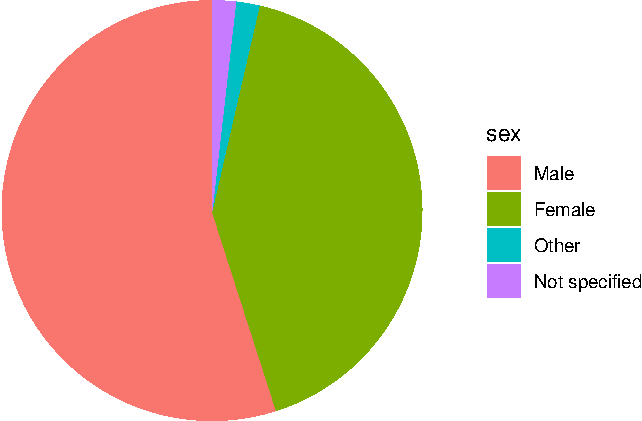
\includegraphics[keepaspectratio]{index_files/figure-pdf/unnamed-chunk-2-1.pdf}}

\textsubscript{Source:
\href{https://matteospanio.github.io/multimodal-symphony-survey-analysis/index.qmd.html}{Article
Notebook}}

}

\subcaption{\label{fig-demographic-info-1}Gender distribution of
participants.}

\end{minipage}%
%
\begin{minipage}{0.50\linewidth}

\centering{

\pandocbounded{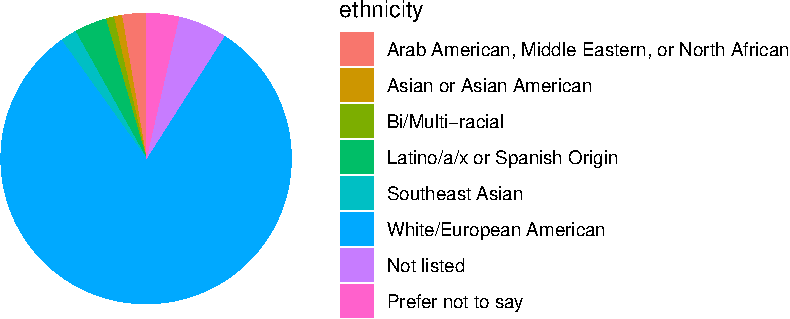
\includegraphics[keepaspectratio]{index_files/figure-pdf/unnamed-chunk-3-1.pdf}}

\textsubscript{Source:
\href{https://matteospanio.github.io/multimodal-symphony-survey-analysis/index.qmd.html}{Article
Notebook}}

}

\subcaption{\label{fig-demographic-info-2}Distribution of participants'
ethnic backgrounds.}

\end{minipage}%
\newline
\begin{minipage}{0.50\linewidth}

\centering{

\pandocbounded{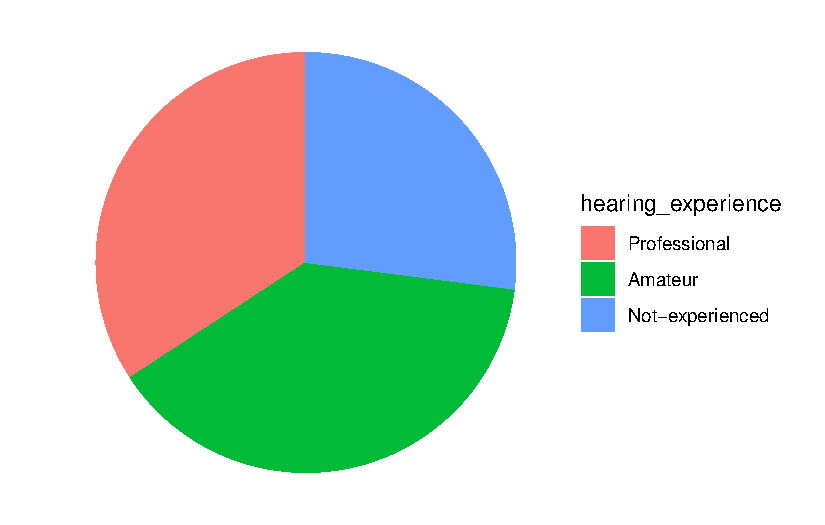
\includegraphics[keepaspectratio]{index_files/figure-pdf/unnamed-chunk-4-1.pdf}}

\textsubscript{Source:
\href{https://matteospanio.github.io/multimodal-symphony-survey-analysis/index.qmd.html}{Article
Notebook}}

}

\subcaption{\label{fig-demographic-info-3}Distribution of participants'
hearing experiences.}

\end{minipage}%
%
\begin{minipage}{0.50\linewidth}

\centering{

\pandocbounded{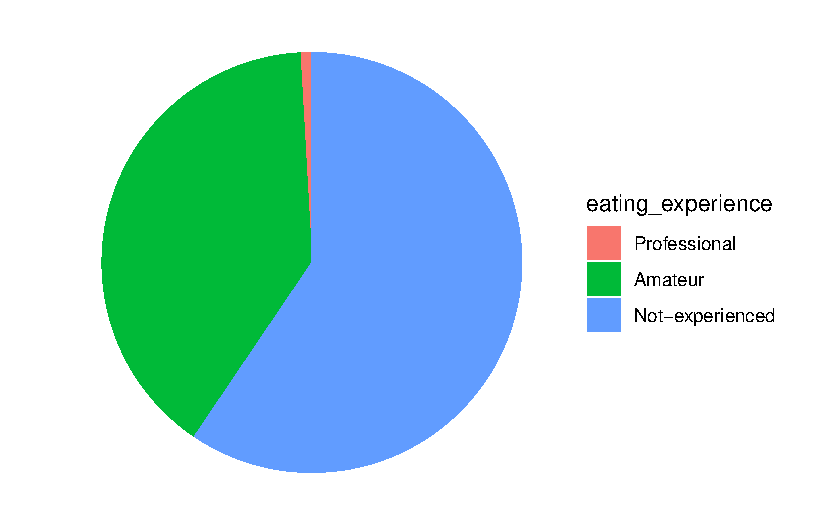
\includegraphics[keepaspectratio]{index_files/figure-pdf/unnamed-chunk-5-1.pdf}}

\textsubscript{Source:
\href{https://matteospanio.github.io/multimodal-symphony-survey-analysis/index.qmd.html}{Article
Notebook}}

}

\subcaption{\label{fig-demographic-info-4}Distribution of participants'
eating experiences.}

\end{minipage}%

\caption{\label{fig-demographic-info}Demographic characteristics of the
study's participants.}

\end{figure}%

Overall the reached population has a mean age of 32 years, whit a
maximum of 75 and a minimum of 19. The mean time spent on the survey was
9 minutes, with a standard deviation of 3.3. Along with age, gender and
execution time also data about musical and eating experience have been
collected: Figure~\ref{fig-demographic-info-2} displays the ethnicity
distribution of the population, the majority of participants recognize
themself as \emph{White/European American}, participants have an almost
equally distributed experience in listening to music (see
Figure~\ref{fig-demographic-info-3}), while just one participant
recognized himself as an experienced eater and the major part of the
sample population declared to be not-experienced in tasting food
(Figure~\ref{fig-demographic-info-4}).

\subsection{Model Preference Analysis}\label{model-preference-analysis}

The first task in the survey involved participants listening to two
audio clips, each corresponding to a taste description chosen randomly
from \emph{sweet}, \emph{sour}, \emph{bitter}, and \emph{salty}. The
goal was to determine which audio sample best matched the given taste
description. The two clips were generated by different versions of the
MusicGEN model {[}2{]}: a fine-tuned version and the original
\footnote{A full description of the model and its finetuning process is
  available at the publication related to this analysis.}, base model,
released by Meta. Participants were asked to express their preference
for the first or second clip by moving a slider ranging from 0 to 10,
where 0 indicated a strong preference for the first clip and 10
indicated a strong preference for the second, Figure~\ref{fig-task1}
shows the survey's first question interface.

\begin{figure}

\centering{

\pandocbounded{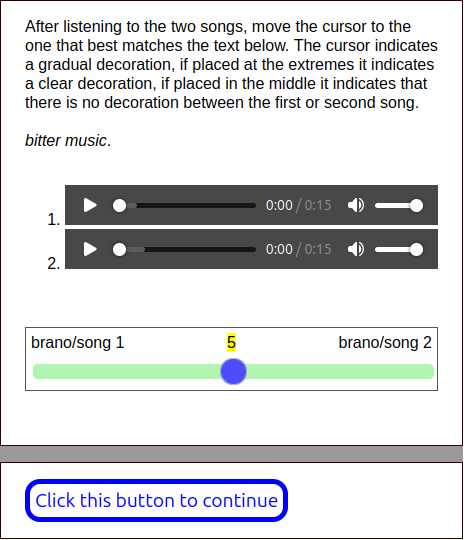
\includegraphics[keepaspectratio]{assets/img/model_preference_woh.png}}

}

\caption{\label{fig-task1}Screenshot of the survey's first task
interface.}

\end{figure}%

To ensure randomization and avoid any bias, the taste descriptions and
audio clips were presented in a random order. In the analysis the scores
are normalized as follows: scores from 0 to 4 are interpreted as a
preference for the base model, scores between 6 and 10 indicate a
preference for the fine-tuned model, and scores of 5 are treated as
neutral.

The underlying research question guiding this task was to assess if the
fine tuned model output better matches taste descriptions than the
sounds generated by the base model.

\subsubsection{Data Visualization}\label{data-visualization}

The distribution of scores across all participants is presented in
Figure~\ref{fig-model-pref-1}. The histogram and density plot show the
spread of scores, allowing us to visually assess the preference for one
model over the other. The base model and fine-tuned model preferences
are expected to manifest as peaks around the lower and higher end of the
score range, respectively.

\begin{figure}

\begin{minipage}{0.50\linewidth}

\centering{

\pandocbounded{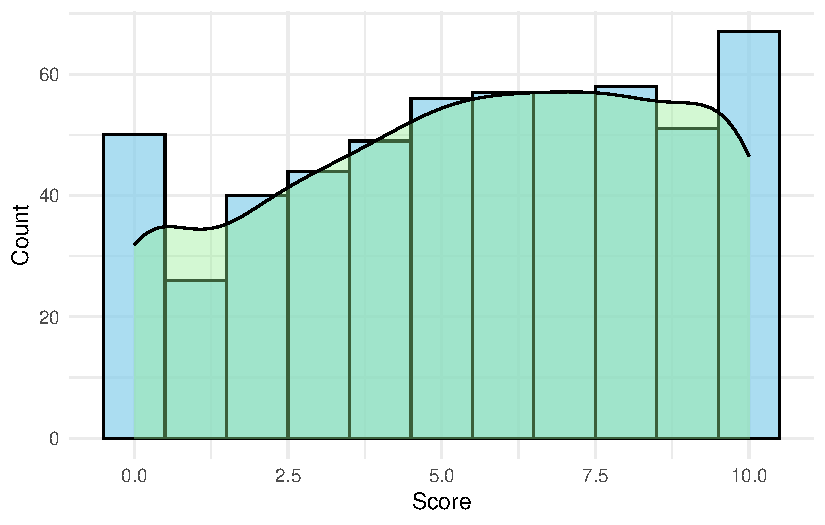
\includegraphics[keepaspectratio]{index_files/figure-pdf/unnamed-chunk-6-1.pdf}}

\textsubscript{Source:
\href{https://matteospanio.github.io/multimodal-symphony-survey-analysis/index.qmd.html}{Article
Notebook}}

}

\subcaption{\label{fig-model-pref-1}Overall evalutation of the models.}

\end{minipage}%
%
\begin{minipage}{0.50\linewidth}

\centering{

\pandocbounded{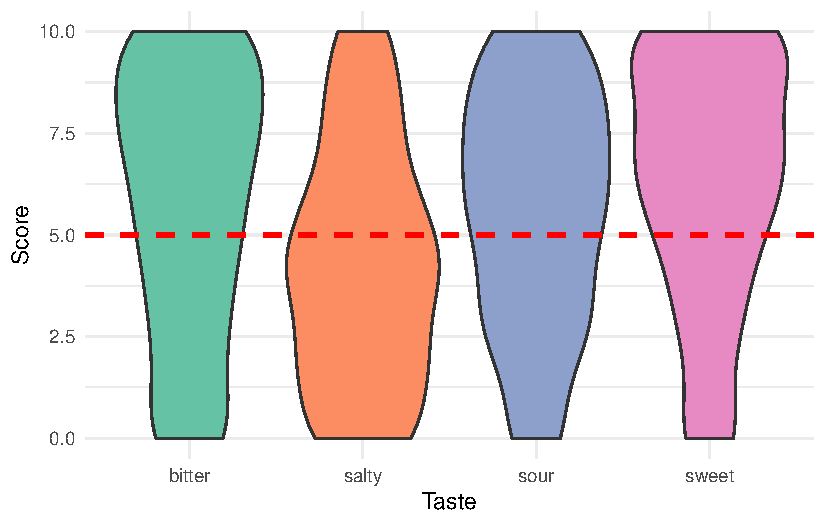
\includegraphics[keepaspectratio]{index_files/figure-pdf/unnamed-chunk-7-1.pdf}}

\textsubscript{Source:
\href{https://matteospanio.github.io/multimodal-symphony-survey-analysis/index.qmd.html}{Article
Notebook}}

}

\subcaption{\label{fig-model-pref-2}Score boxplot by taste category.}

\end{minipage}%
\newline
\begin{minipage}{\linewidth}

\centering{

\pandocbounded{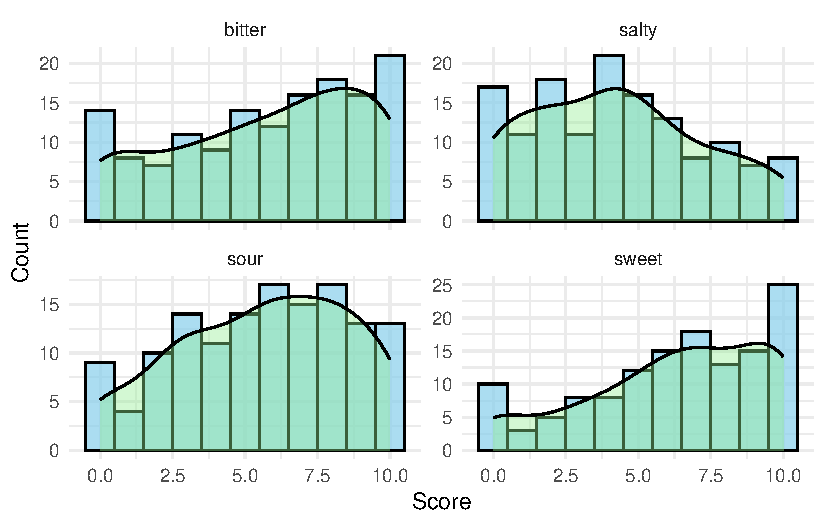
\includegraphics[keepaspectratio]{index_files/figure-pdf/unnamed-chunk-8-1.pdf}}

\textsubscript{Source:
\href{https://matteospanio.github.io/multimodal-symphony-survey-analysis/index.qmd.html}{Article
Notebook}}

}

\subcaption{\label{fig-model-pref-3}Score distribution by taste
category.}

\end{minipage}%

\caption{\label{fig-model-pref}Score distribution between the two
models.}

\end{figure}%

Figure~\ref{fig-model-pref-2} goes further by breaking down the
preferences based on the taste category described in the audio sample.
Each taste category is visualized using boxplots, where the median score
for each taste can be assessed. This enables us to examine whether the
model preference varies depending on the taste label, with the red
dashed line at a score of 5 acting as the neutral threshold.

\subsubsection{Hypothesis Testing}\label{hypothesis-testing}

Next, we assess whether the average score for the audio samples
significantly differs from a neutral score of 5, under the assumption
that the preference for the fine-tuned model should be greater than this
threshold. To do this, we need to verify whether the data follows a
normal distribution. In order to assess normality of data we applied
both visual and computational methods, then firstly a Q-Q plot was
generated to visually inspect the normality of the score distribution,
see Figure~\ref{fig-qqplot}. The resulting plot shows deviations from
the expected straight line, indicating that the scores do not follow a
normal distribution.

\phantomsection\label{cell-fig-qqplot}
\begin{figure}[H]

\centering{

\pandocbounded{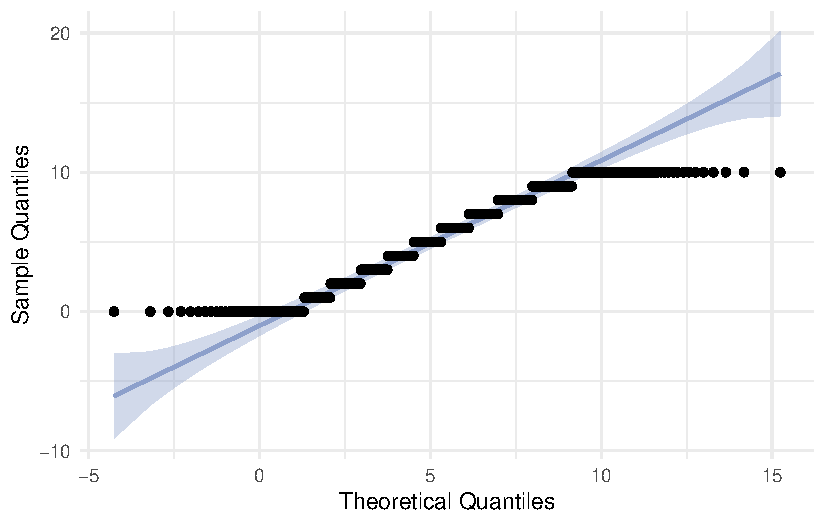
\includegraphics[keepaspectratio]{index_files/figure-pdf/fig-qqplot-1.pdf}}

}

\caption{\label{fig-qqplot}Q-Q plot to assess the normality distribution
of the collected data.}

\end{figure}%

\textsubscript{Source:
\href{https://matteospanio.github.io/multimodal-symphony-survey-analysis/index.qmd.html}{Article
Notebook}}

\textsubscript{Source:
\href{https://matteospanio.github.io/multimodal-symphony-survey-analysis/index.qmd.html}{Article
Notebook}}

In addition the Shapiro-Wilk test confirmed that the data significantly
deviate from a normal distribution (with a resulting \(p\)-value equals
to \(\ensuremath{2.516\times 10^{-14}}\)). Therefore, we decide to apply
the non-parametric Wilcoxon signed-rank test to see if the models
preference score expressed by participants has a mean major than the
null preference (score equals to five), more formally we are testing the
hypothesis:

\[
H_0: \mu = 5 \quad H_1: \mu > 5
\] where \(H_0\) means that there is no preference between the two
models while \(H_1\) means that the fine-tuned model is preferred over
the other one with a \(95%
\) confidence interval.

\textsubscript{Source:
\href{https://matteospanio.github.io/multimodal-symphony-survey-analysis/index.qmd.html}{Article
Notebook}}

The result of the Wilcoxon test shows a \(p\)-value of
\(\ensuremath{1.498\times 10^{-4}}\), which is less than \(0.05\),
indicating that we can reject the null hypothesis and conclude that the
median score is indeed significantly greater than \(5\). This supports
the hypothesis that the participants prefer the fine-tuned model
overall.

\subsubsection{Post-Hoc Analysis by
Taste}\label{post-hoc-analysis-by-taste}

While the Wilcoxon test confirms that the overall preference goes to the
fine-tuned model the boxplots reveal a variation of the score by taste,
to confirm the variation we perform separate Wilcoxon tests for each
taste group (\emph{sweet}, \emph{sour}, \emph{bitter}, \emph{salty}). We
use a Bonferroni correction to adjust for the multiple comparisons and
control the family-wise error rate. The results of the post-hoc tests
are shown below, in Table~\ref{tbl-wilcoxon-taste}.

\begin{longtable}[]{@{}lrr@{}}

\caption{\label{tbl-wilcoxon-taste}Results of the Wilcoxon test
performed on data filtered by taste.}

\tabularnewline

\toprule\noalign{}
& p.value & adjusted.p.value \\
\midrule\noalign{}
\endhead
\bottomrule\noalign{}
\endlastfoot
bitter & 0.0034381 & 0.0137523 \\
salty & 0.9969070 & 1.0000000 \\
sour & 0.0076040 & 0.0304159 \\
sweet & 0.0000043 & 0.0000171 \\

\end{longtable}

\textsubscript{Source:
\href{https://matteospanio.github.io/multimodal-symphony-survey-analysis/index.qmd.html}{Article
Notebook}}

The analysis reveals that the fine-tuned model was significantly
preferred for the sweet taste category, with an adjusted \(p\)-value of
\(\ensuremath{1.7060421\times 10^{-5}}\), well below the conventional
threshold of \(0.05\). This suggests a strong alignment between the
musical outputs and participants' expectations of sweetness. Conversely,
the bitter and sour categories also exhibited significant preferences,
with adjusted \(p\)-values of \(0.0137523\) and \(0.0304159\),
respectively. However, these results, while statistically significant,
indicate a less robust preference compared to the sweet category.
Notably, the salty taste group did not demonstrate a significant
preference for the fine-tuned model, as indicated by an adjusted
\(p\)-value near to 1. This lack of significance suggests that the
model's performance may not align with participants' expectations for
salty flavors, warranting further investigation into the underlying
factors influencing this outcome.

\textsubscript{Source:
\href{https://matteospanio.github.io/multimodal-symphony-survey-analysis/index.qmd.html}{Article
Notebook}}

Since the finetuned model did not show to perform well on the salty
group, we performed a Wilcoxon test to test if its mean is significally
lower than the tie situation
(\(H_0: \mu_{\text{salty}} = 5, H_1: \mu_{\text{salty}} < 5\)) the
result is that the first model is statistically preferred over the
finetuned variant according to the Wilcoxon test with a \(p\)-value
equal to \(0.0031167\) without Bonferroni correction\footnote{The
  Bonferroni correction has not been applied due to the non indepenent
  nature of the test, in fact the test has been performed after the
  results of the previous Wilcoxon test, which, instead, was testing
  independently 4 groups.}.

\subsection{Recognisability of Tastes}\label{recognisability-of-tastes}

In the second task of the survey, participants were asked to listen to
musical pieces generated exclusively by the fine-tuned model to better
investigate the intrinsic qualities carried by the generated music.
Following each listening session, participants were required to quantify
the flavors they perceived in the music using a graduated scale, ranging
from 1 to 5 (where 1 means \emph{not at all} and 5 means \emph{very
much}), for each of the four primary taste categories: salty, sweet,
bitter, and sour. Unlike the first task, there were no imposed labels
for specific flavors, allowing participants the freedom to associate
values with each taste based on their personal interpretations of the
musical experience. Additionally, to enrich the assessment, participants
had to evaluate their emotional responses to the music by rating various
non-gustatory parameters, including happiness, sadness, anger, disgust,
fear, surprise, hot, and cold. Figure~\ref{fig-task2} displays the web
interface used to collect participants' responses.

\begin{figure}

\centering{

\pandocbounded{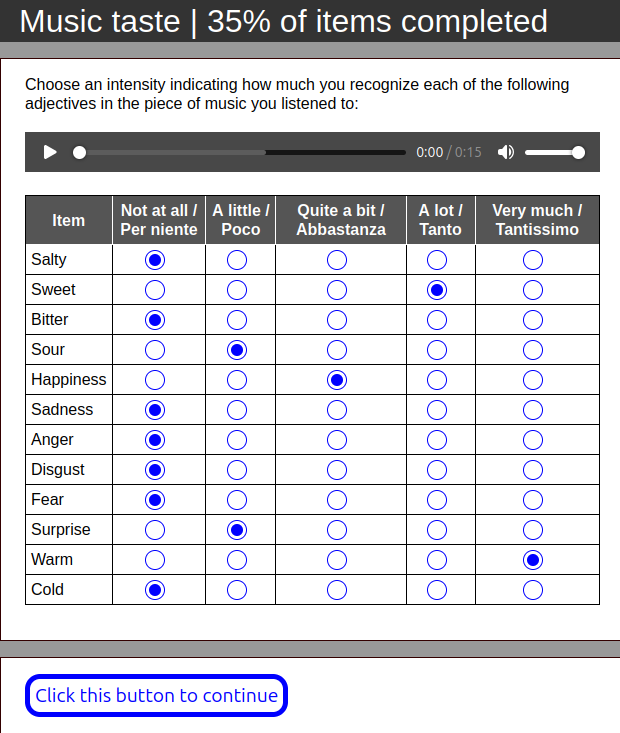
\includegraphics[keepaspectratio]{assets/img/music_synesthesia.png}}

}

\caption{\label{fig-task2}Screenshot of the survey's second task
interface.}

\end{figure}%

The underlying research questions guiding this task were:

\begin{enumerate}
\def\labelenumi{\arabic{enumi}.}
\tightlist
\item
  Can the music generated by the model induce sensory-gustatory
  responses?
\item
  What correlations exist between music and taste?
\item
  Which emotions mediate these sensory responses?
\end{enumerate}

\subsubsection{ANOVA test}\label{anova-test}

To address the first research question, we performed an Analysis of
Variance (ANOVA) to evaluate whether the participants' ratings of
stimuli varied according to distinct stimulus characteristics. The
dependent variable was the value assigned by participants to each
stimulus, while the independent variables included stimulus-related
factors. The dataset was filtered to include only participants
identifying as \emph{Male} or \emph{Female}, excluding participants
classified as \emph{Professional Eaters} due to insufficient
representation of this category. This preprocessing step ensured robust
and meaningful comparisons between groups.

\begin{longtable}[]{@{}lrrrrr@{}}

\caption{\label{tbl-anova-value}Results of the ANOVA test.}

\tabularnewline

\toprule\noalign{}
& Df & Sum Sq & Mean Sq & F value & Pr(\textgreater F) \\
\midrule\noalign{}
\endhead
\bottomrule\noalign{}
\endlastfoot
prompt & 3 & 29.402 & 9.801 & 8.739 & 0.000 \\
adjective & 11 & 188.478 & 17.134 & 15.279 & 0.000 \\
hearing\_experience & 2 & 37.299 & 18.650 & 16.630 & 0.000 \\
eating\_experience & 1 & 0.711 & 0.711 & 0.634 & 0.426 \\
sex & 1 & 0.069 & 0.069 & 0.061 & 0.804 \\
prompt:adjective & 33 & 214.757 & 6.508 & 5.803 & 0.000 \\
Residuals & 3764 & 4221.057 & 1.121 & NA & NA \\

\end{longtable}

\textsubscript{Source:
\href{https://matteospanio.github.io/multimodal-symphony-survey-analysis/index.qmd.html}{Article
Notebook}}

The results of the ANOVA are summarized in Table~\ref{tbl-anova-value},
which presents the degrees of freedom (Df), sum of squares (Sum Sq),
mean squares (Mean Sq), F-statistics, and \(p\)-values for each factor
and interaction.

Prior to interpreting the results, the homoskedasticity assumption was
assessed by examining the residuals. A Shapiro-Wilk test indicated
evidence of heteroskedasticity (\(p < 0.05\)). Despite this violation,
the ANOVA analysis proceeded, following recommendations from prior
research {[}3{]}, {[}4{]}, {[}5{]} suggesting that ANOVA is robust to
deviations from normality under moderate violations, particularly with
large sample sizes such as the one in this study. The results show that
different prompts and adjectives lead to significantly different
adjectives quantified by participants, similarly the adjectives used
influence the participants' feelings. Furthermore the significant
interaction effect implies that the effect of one variable depends on
the level of the other. In other words, the way a prompt influences
feelings may vary depending on the adjective used. This result
highlights that the participants to the survey deliberately operated
consistent choices while evaluating the stimuli.

\subsubsection{Post-Hoc Analysis}\label{post-hoc-analysis}

To further explore the results of the ANOVA, we conducted Tukey's Honest
Significant Difference (HSD) test. This post-hoc analysis is
particularly useful for identifying which specific group means are
significantly different from each other after finding a significant
overall effect in the ANOVA. Given that our analysis revealed
significant main effects for prompt, adjective, their interaction and
the hearing experience, it is essential to determine the nature of these
differences.

The Tukey test compares all possible pairs of group means while
controlling for the family-wise error rate, thus providing a robust
method for multiple comparisons. This is crucial in our context, as we
aim to understand how different prompts, adjectives and hearing
experience levels influence participants' evaluations of the stimuli.
Upon executing the Tukey test, we examined the adjusted \(p\)-values for
each comparison. The results indicated several significant differences
between specific combinations of prompts and adjectives, as summarized
in the table below:

\textsubscript{Source:
\href{https://matteospanio.github.io/multimodal-symphony-survey-analysis/index.qmd.html}{Article
Notebook}}

\begin{longtable}[]{@{}lrrrr@{}}
\caption{Tukey test between different prompts with a \(p\)-value lower
0.05.}\tabularnewline
\toprule\noalign{}
& diff & lwr & upr & p adj \\
\midrule\noalign{}
\endfirsthead
\toprule\noalign{}
& diff & lwr & upr & p adj \\
\midrule\noalign{}
\endhead
\bottomrule\noalign{}
\endlastfoot
sour-bitter & 0.1539030 & 0.0274663 & 0.2803397 & 0.0095792 \\
sour-salty & 0.1942878 & 0.0661296 & 0.3224460 & 0.0005747 \\
sweet-sour & -0.1932957 & -0.3214540 & -0.0651375 & 0.0006229 \\
\end{longtable}

\textsubscript{Source:
\href{https://matteospanio.github.io/multimodal-symphony-survey-analysis/index.qmd.html}{Article
Notebook}}

\begin{longtable}[]{@{}lrrrr@{}}
\caption{Tukey test between different adjectives with a \(p\)-value
lower 0.05.}\tabularnewline
\toprule\noalign{}
& diff & lwr & upr & p adj \\
\midrule\noalign{}
\endfirsthead
\toprule\noalign{}
& diff & lwr & upr & p adj \\
\midrule\noalign{}
\endhead
\bottomrule\noalign{}
\endlastfoot
bitter-anger & 0.4204204 & 0.1439129 & 0.6969280 & 0.0000443 \\
cold-anger & 0.4774775 & 0.2009699 & 0.7539850 & 0.0000012 \\
hot-anger & 0.5315315 & 0.2550240 & 0.8080391 & 0.0000000 \\
sad-anger & 0.5765766 & 0.3000690 & 0.8530841 & 0.0000000 \\
sweet-anger & 0.3723724 & 0.0958648 & 0.6488799 & 0.0006699 \\
disgust-bitter & -0.6336336 & -0.9101412 & -0.3571261 & 0.0000000 \\
happy-bitter & -0.3093093 & -0.5858169 & -0.0328018 & 0.0136899 \\
surprise-bitter & -0.2852853 & -0.5617928 & -0.0087777 & 0.0360645 \\
disgust-cold & -0.6906907 & -0.9671982 & -0.4141831 & 0.0000000 \\
happy-cold & -0.3663664 & -0.6428739 & -0.0898588 & 0.0009180 \\
sour-cold & -0.2852853 & -0.5617928 & -0.0087777 & 0.0360645 \\
surprise-cold & -0.3423423 & -0.6188499 & -0.0658348 & 0.0030580 \\
fear-disgust & 0.4324324 & 0.1559249 & 0.7089400 & 0.0000213 \\
happy-disgust & 0.3243243 & 0.0478168 & 0.6008319 & 0.0070884 \\
hot-disgust & 0.7447447 & 0.4682372 & 1.0212523 & 0.0000000 \\
sad-disgust & 0.7897898 & 0.5132822 & 1.0662973 & 0.0000000 \\
salty-disgust & 0.4684685 & 0.1919609 & 0.7449760 & 0.0000021 \\
sour-disgust & 0.4054054 & 0.1288979 & 0.6819130 & 0.0001074 \\
surprise-disgust & 0.3483483 & 0.0718408 & 0.6248559 & 0.0022833 \\
sweet-disgust & 0.5855856 & 0.3090780 & 0.8620931 & 0.0000000 \\
hot-fear & 0.3123123 & 0.0358048 & 0.5888199 & 0.0120394 \\
sad-fear & 0.3573574 & 0.0808498 & 0.6338649 & 0.0014571 \\
hot-happy & 0.4204204 & 0.1439129 & 0.6969280 & 0.0000443 \\
sad-happy & 0.4654655 & 0.1889579 & 0.7419730 & 0.0000026 \\
sour-hot & -0.3393393 & -0.6158469 & -0.0628318 & 0.0035312 \\
surprise-hot & -0.3963964 & -0.6729040 & -0.1198888 & 0.0001798 \\
salty-sad & -0.3213213 & -0.5978289 & -0.0448138 & 0.0081111 \\
sour-sad & -0.3843844 & -0.6608919 & -0.1078768 & 0.0003509 \\
surprise-sad & -0.4414414 & -0.7179490 & -0.1649339 & 0.0000122 \\
\end{longtable}

\textsubscript{Source:
\href{https://matteospanio.github.io/multimodal-symphony-survey-analysis/index.qmd.html}{Article
Notebook}}

\begin{longtable}[]{@{}
  >{\raggedright\arraybackslash}p{(\linewidth - 8\tabcolsep) * \real{0.3582}}
  >{\raggedleft\arraybackslash}p{(\linewidth - 8\tabcolsep) * \real{0.1642}}
  >{\raggedleft\arraybackslash}p{(\linewidth - 8\tabcolsep) * \real{0.1642}}
  >{\raggedleft\arraybackslash}p{(\linewidth - 8\tabcolsep) * \real{0.1642}}
  >{\raggedleft\arraybackslash}p{(\linewidth - 8\tabcolsep) * \real{0.1493}}@{}}
\caption{Tukey test between different hearing experience groups with a
\(p\)-value lower 0.05.}\tabularnewline
\toprule\noalign{}
\begin{minipage}[b]{\linewidth}\raggedright
\end{minipage} & \begin{minipage}[b]{\linewidth}\raggedleft
diff
\end{minipage} & \begin{minipage}[b]{\linewidth}\raggedleft
lwr
\end{minipage} & \begin{minipage}[b]{\linewidth}\raggedleft
upr
\end{minipage} & \begin{minipage}[b]{\linewidth}\raggedleft
p adj
\end{minipage} \\
\midrule\noalign{}
\endfirsthead
\toprule\noalign{}
\begin{minipage}[b]{\linewidth}\raggedright
\end{minipage} & \begin{minipage}[b]{\linewidth}\raggedleft
diff
\end{minipage} & \begin{minipage}[b]{\linewidth}\raggedleft
lwr
\end{minipage} & \begin{minipage}[b]{\linewidth}\raggedleft
upr
\end{minipage} & \begin{minipage}[b]{\linewidth}\raggedleft
p adj
\end{minipage} \\
\midrule\noalign{}
\endhead
\bottomrule\noalign{}
\endlastfoot
Amateur-Professional & 0.2268160 & 0.1318865 & 0.3217454 & 0.0000001 \\
Not-experienced-Amateur & -0.1684003 & -0.2698267 & -0.0669739 &
0.0002967 \\
\end{longtable}

\textsubscript{Source:
\href{https://matteospanio.github.io/multimodal-symphony-survey-analysis/index.qmd.html}{Article
Notebook}}

These significant comparisons illuminate the subtleties in participants'
responses to different stimuli. Certain prompt-adjective combinations
elicited stronger emotional reactions than others, indicating that the
interaction between prompts and adjectives significantly shapes
participants' perceptions. Notably, some combinations yielded adjusted
\(p\)-values below the conventional threshold of \(0.05\), signifying
statistically significant differences. This finding reinforces the ANOVA
results, confirming that the presentation of prompts and adjectives can
meaningfully impact emotional responses.

\subsubsection{\texorpdfstring{Interaction between \emph{prompt} and
\emph{adjective}}{Interaction between prompt and adjective}}\label{interaction-between-prompt-and-adjective}

The ANOVA analysis evidenced also a significant interaction between
prompt and adjectives used to evaluate the sounds, as we know, the
design of the experiment fixed the prompt before generating the audio
files, therefore adjectives has to be intended as dependent variables
while the prompts are independent; in other words, participants assigned
different values to the adjectives to the sounds on the basis of their
generation prompt. This interaction can be seen in
Figure~\ref{fig-heatmap}. In particular Figure~\ref{fig-heatmap-taste}
shows the mean value assigned to each taste adjective by their prompt,
we can clearly seen the major diagonal emerge by the \(4 \times 4\)
matrix, this means that, the mean value assigned to the adjective that
matches the prompt of each sound is the highest. The rest of the
interaction between adjectives and prompt can be seen in
Figure~\ref{fig-heatmap-emotions} , a deeper analysis of emotional
aspect assigned to the sounds is presented in the next section.

\begin{figure}

\begin{minipage}{0.50\linewidth}

\centering{

\pandocbounded{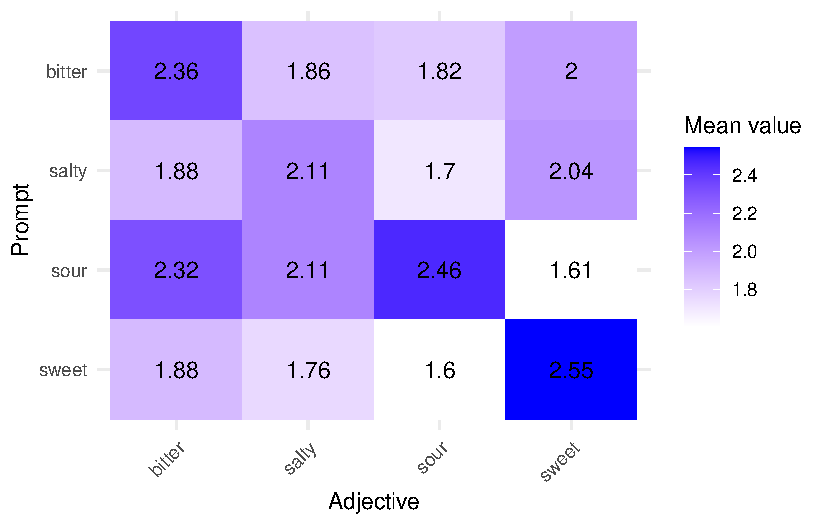
\includegraphics[keepaspectratio]{index_files/figure-pdf/unnamed-chunk-19-1.pdf}}

\textsubscript{Source:
\href{https://matteospanio.github.io/multimodal-symphony-survey-analysis/index.qmd.html}{Article
Notebook}}

}

\subcaption{\label{fig-heatmap-taste}Heatmap of perceived taste in
correspondence of the intended one.}

\end{minipage}%
%
\begin{minipage}{0.50\linewidth}

\centering{

\pandocbounded{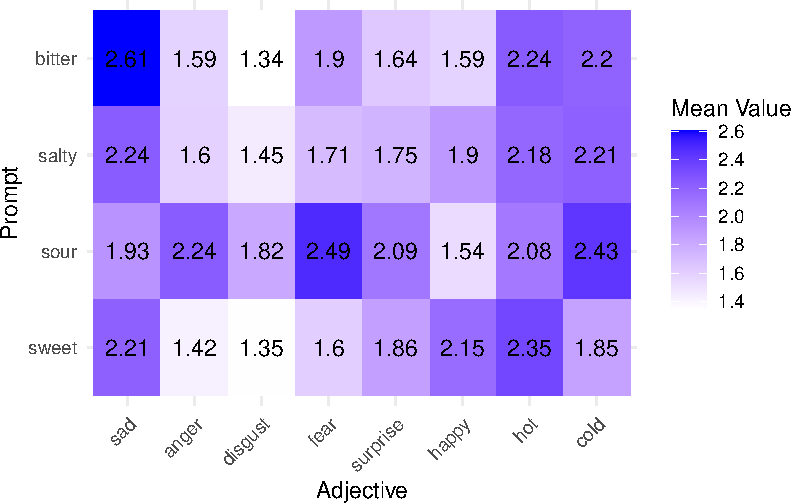
\includegraphics[keepaspectratio]{index_files/figure-pdf/unnamed-chunk-20-1.pdf}}

\textsubscript{Source:
\href{https://matteospanio.github.io/multimodal-symphony-survey-analysis/index.qmd.html}{Article
Notebook}}

}

\subcaption{\label{fig-heatmap-emotions}Heatmap of perceived emotional
response in correspondence of the suggested taste.}

\end{minipage}%

\caption{\label{fig-heatmap}Heatmaps}

\end{figure}%

\subsubsection{Factorial analysis}\label{factorial-analysis}

\textsubscript{Source:
\href{https://matteospanio.github.io/multimodal-symphony-survey-analysis/index.qmd.html}{Article
Notebook}}

To explore the underlying relationships between sensory qualities and
emotional states, we conducted a factor analysis on the standardized
data, excluding the `taste' column. The initial step involved
calculating the correlation matrix, which revealed notable relationships
among the adjectives. Specifically, we observed that negative emotions
were positively correlated, while the pair happy-sad exhibited a
negative correlation. Furthermore, sweetness demonstrated a strong
correlation with happiness and warmth, whereas bitterness was associated
with anger and fear. Sourness, on the other hand, was evidently
correlated with disgust and fear. Other variables did not show strong
correlations at first glance, prompting us to proceed with the factor
analysis.

\phantomsection\label{cell-fig-corr-matrix}
\begin{figure}[H]

\centering{

\pandocbounded{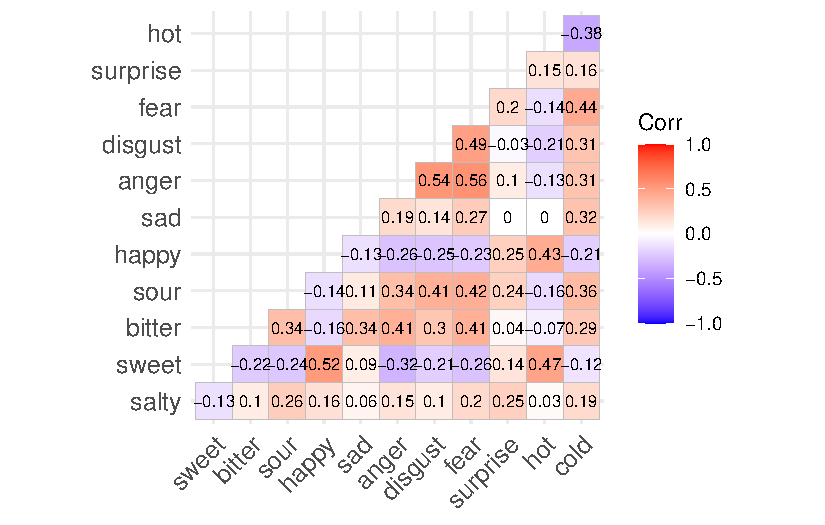
\includegraphics[keepaspectratio]{index_files/figure-pdf/fig-corr-matrix-1.pdf}}

}

\caption{\label{fig-corr-matrix}Correlation matrix}

\end{figure}%

\textsubscript{Source:
\href{https://matteospanio.github.io/multimodal-symphony-survey-analysis/index.qmd.html}{Article
Notebook}}

The correlation matrix is illustrated in Figure~\ref{fig-corr-matrix},
showcasing these relationships clearly.

\phantomsection\label{cell-fig-scree-plots}
\begin{verbatim}
Parallel analysis suggests that the number of factors =  4  and the number of components =  NA 
\end{verbatim}

\begin{figure}[H]

\centering{

\pandocbounded{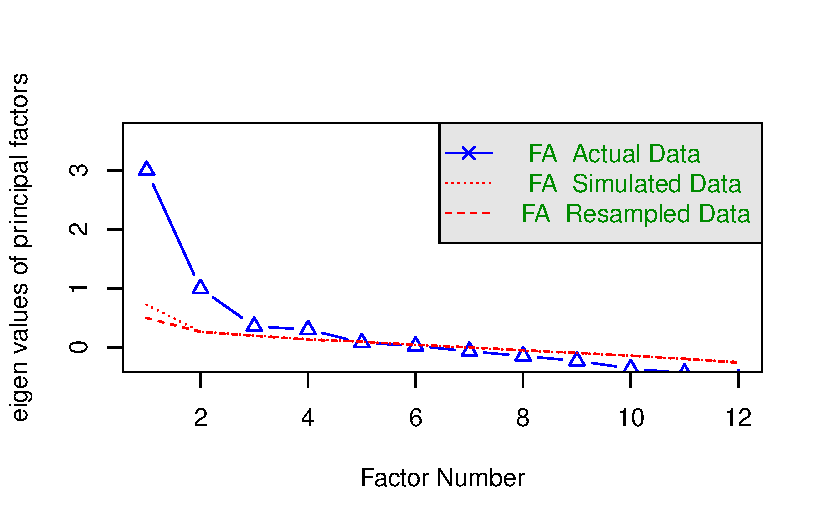
\includegraphics[keepaspectratio]{index_files/figure-pdf/fig-scree-plots-1.pdf}}

}

\caption{\label{fig-scree-plots}Parallel Analysis Scree Plots}

\end{figure}%

\textsubscript{Source:
\href{https://matteospanio.github.io/multimodal-symphony-survey-analysis/index.qmd.html}{Article
Notebook}}

To determine the optimal number of factors for our analysis, we employed
parallel analysis, which indicated an optimal number of 4 factors. This
estimation serves as a foundation for our subsequent factor analysis.
Following this, we executed the factor analysis using the identified
number of factors, applying an oblique rotation (oblimin) to allow for
potential correlations among the factors. The results of the factor
analysis, including the factor loadings, are presented in the output.
The factor loadings indicate how strongly each variable contributes to
the identified factors, providing insights into the underlying structure
of the data.

\phantomsection\label{cell-fig-factor-analysis}
\begin{figure}[H]

\centering{

\pandocbounded{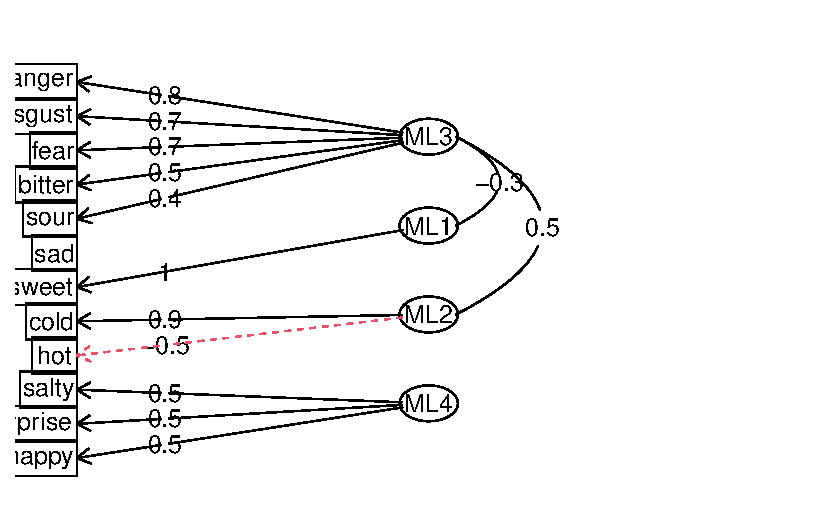
\includegraphics[keepaspectratio]{index_files/figure-pdf/fig-factor-analysis-1.pdf}}

}

\caption{\label{fig-factor-analysis}Factor analysis graph.}

\end{figure}%

\textsubscript{Source:
\href{https://matteospanio.github.io/multimodal-symphony-survey-analysis/index.qmd.html}{Article
Notebook}}

\begin{verbatim}

Loadings:
         ML3    ML1    ML2    ML4   
salty           -0.231  0.111  0.535
sweet            0.992              
bitter    0.502                     
sour      0.385 -0.128  0.178  0.226
happy    -0.197  0.302 -0.132  0.492
sad       0.292  0.259  0.236       
anger     0.779                     
disgust   0.694               -0.133
fear      0.662         0.133  0.113
surprise                0.120  0.526
hot       0.140  0.361 -0.458  0.267
cold                    0.882       

                 ML3   ML1   ML2   ML4
SS loadings    2.083 1.360 1.146 0.971
Proportion Var 0.174 0.113 0.096 0.081
Cumulative Var 0.174 0.287 0.382 0.463
\end{verbatim}

\textsubscript{Source:
\href{https://matteospanio.github.io/multimodal-symphony-survey-analysis/index.qmd.html}{Article
Notebook}}

To visualize the relationships among the factors, we generated biplots
for various factor combinations. The biplots, shown in the subsequent
figures, illustrate the distribution of variables across the identified
factors, highlighting the clustering of adjectives associated with
similar emotional states.

\begin{figure}

\begin{minipage}{0.50\linewidth}

\centering{

\pandocbounded{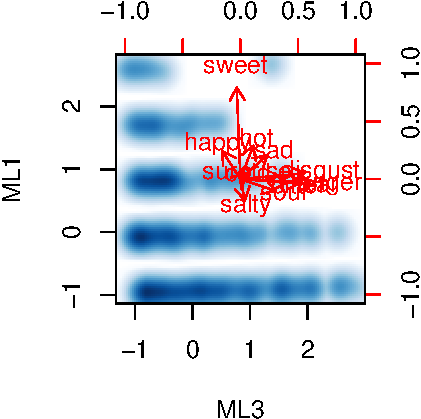
\includegraphics[keepaspectratio]{index_files/figure-pdf/unnamed-chunk-26-1.pdf}}

\textsubscript{Source:
\href{https://matteospanio.github.io/multimodal-symphony-survey-analysis/index.qmd.html}{Article
Notebook}}

}

\subcaption{\label{fig-fa-biplot-1}}

\end{minipage}%
%
\begin{minipage}{0.50\linewidth}

\centering{

\pandocbounded{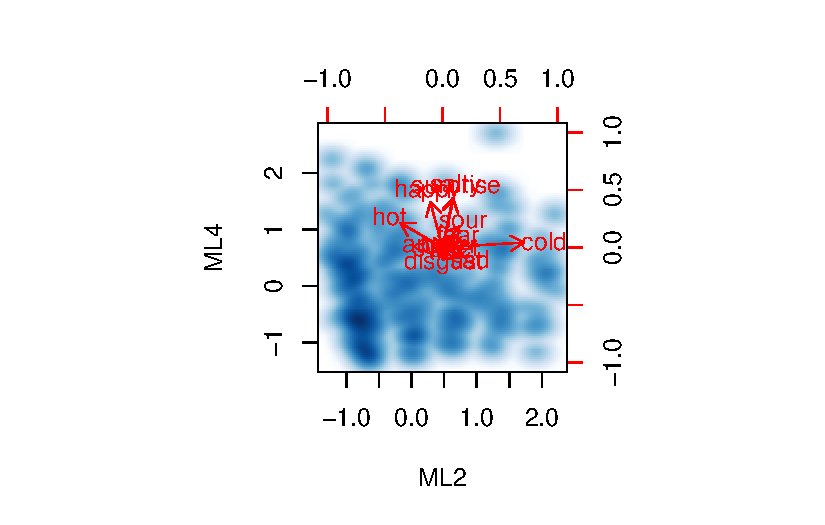
\includegraphics[keepaspectratio]{index_files/figure-pdf/unnamed-chunk-27-1.pdf}}

\textsubscript{Source:
\href{https://matteospanio.github.io/multimodal-symphony-survey-analysis/index.qmd.html}{Article
Notebook}}

}

\subcaption{\label{fig-fa-biplot-2}}

\end{minipage}%
\newline
\begin{minipage}{0.50\linewidth}

\centering{

\pandocbounded{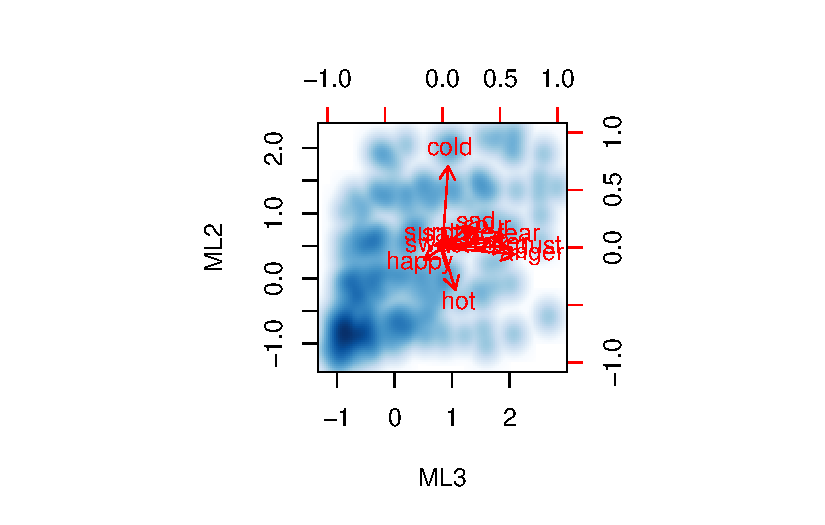
\includegraphics[keepaspectratio]{index_files/figure-pdf/unnamed-chunk-28-1.pdf}}

\textsubscript{Source:
\href{https://matteospanio.github.io/multimodal-symphony-survey-analysis/index.qmd.html}{Article
Notebook}}

}

\subcaption{\label{fig-fa-biplot-3}}

\end{minipage}%
%
\begin{minipage}{0.50\linewidth}

\centering{

\pandocbounded{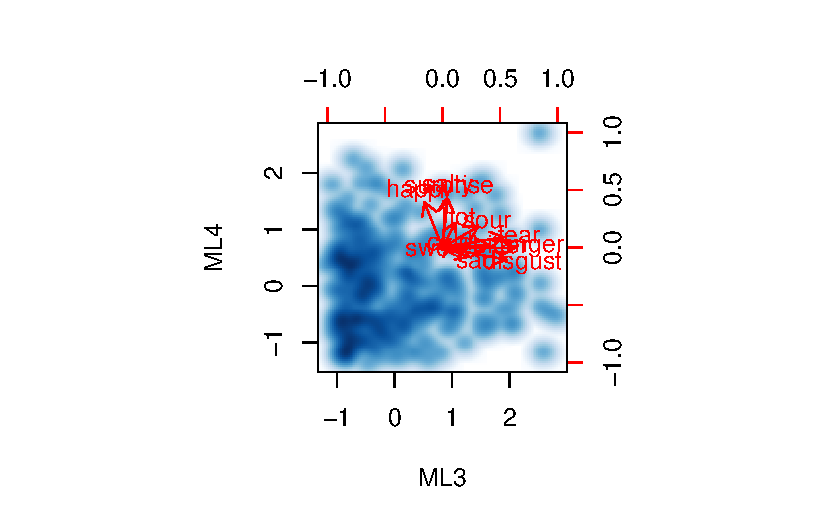
\includegraphics[keepaspectratio]{index_files/figure-pdf/unnamed-chunk-29-1.pdf}}

\textsubscript{Source:
\href{https://matteospanio.github.io/multimodal-symphony-survey-analysis/index.qmd.html}{Article
Notebook}}

}

\subcaption{\label{fig-fa-biplot-4}}

\end{minipage}%

\caption{\label{fig-fa-biplot}Loadings biplot over the four factors.}

\end{figure}%

\begin{longtable}[]{@{}
  >{\raggedright\arraybackslash}p{(\linewidth - 8\tabcolsep) * \real{0.0609}}
  >{\raggedright\arraybackslash}p{(\linewidth - 8\tabcolsep) * \real{0.2348}}
  >{\raggedright\arraybackslash}p{(\linewidth - 8\tabcolsep) * \real{0.2348}}
  >{\raggedright\arraybackslash}p{(\linewidth - 8\tabcolsep) * \real{0.2348}}
  >{\raggedright\arraybackslash}p{(\linewidth - 8\tabcolsep) * \real{0.2348}}@{}}
\toprule\noalign{}
\begin{minipage}[b]{\linewidth}\raggedright
Prompt
\end{minipage} & \begin{minipage}[b]{\linewidth}\raggedright
Fattore 1
\end{minipage} & \begin{minipage}[b]{\linewidth}\raggedright
Fattore 2
\end{minipage} & \begin{minipage}[b]{\linewidth}\raggedright
Fattore 3
\end{minipage} & \begin{minipage}[b]{\linewidth}\raggedright
Fattore 4
\end{minipage} \\
\midrule\noalign{}
\endhead
\bottomrule\noalign{}
\endlastfoot
bitter & \(\mu=-0.01\), \(\sigma=0.82\) & \(\mu=-0.06\), \(\sigma=0.99\)
& \(\mu=0.04\), \(\sigma=0.91\) & \(\mu=-0.16\), \(\sigma=0.69\) \\
salty & \(\mu=-0.13\), \(\sigma=0.87\) & \(\mu=-0.03\), \(\sigma=0.98\)
& \(\mu=0.01\), \(\sigma=0.94\) & \(\mu=0.02\), \(\sigma=0.94\) \\
sour & \(\mu=0.50\), \(\sigma=1.02\) & \(\mu=-0.39\), \(\sigma=0.79\) &
\(\mu=0.23\), \(\sigma=0.93\) & \(\mu=0.11\), \(\sigma=0.74\) \\
sweet & \(\mu=-0.30\), \(\sigma=0.74\) & \(\mu=0.43\), \(\sigma=1.04\) &
\(\mu=-0.26\), \(\sigma=0.82\) & \(\mu=0.05\), \(\sigma=0.80\) \\
\end{longtable}

\textsubscript{Source:
\href{https://matteospanio.github.io/multimodal-symphony-survey-analysis/index.qmd.html}{Article
Notebook}}

Lastly, we performed a multi-factor analysis to further explore the
dimensions of negativity and positivity within the data. The results of
this analysis are depicted in the multi-factor diagram, which
categorizes the factors into two overarching themes: Negativity and
Positivity.

\begin{figure}

\centering{

\pandocbounded{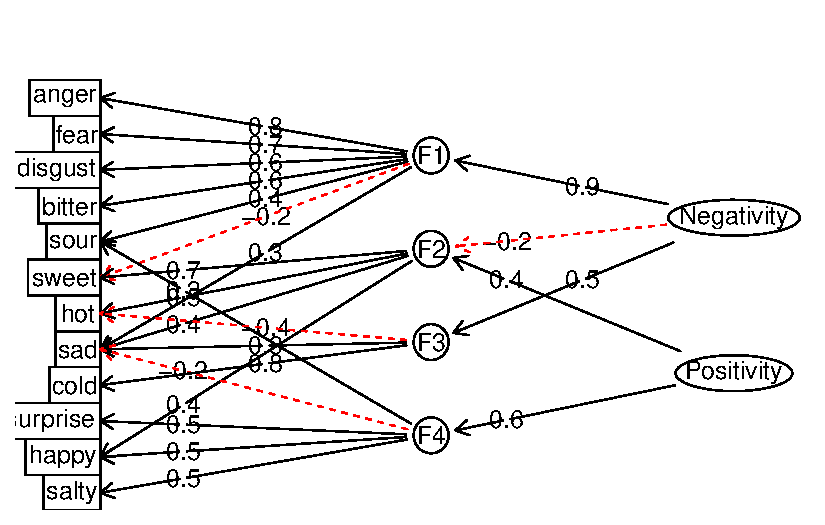
\includegraphics[keepaspectratio]{index_files/figure-pdf/unnamed-chunk-31-1.pdf}}

\textsubscript{Source:
\href{https://matteospanio.github.io/multimodal-symphony-survey-analysis/index.qmd.html}{Article
Notebook}}

}

\caption{\label{fig-multilevel-fa}Hierarchical (multilevel) factors'
structure.}

\end{figure}%

\subsection{References}\label{references}

\phantomsection\label{refs}
\begin{CSLReferences}{0}{0}
\bibitem[\citeproctext]{ref-stoet_psytoolkit_2017}
\CSLLeftMargin{{[}1{]} }%
\CSLRightInline{G. Stoet, {``PsyToolkit: A novel web-based method for
running online questionnaires and reaction-time experiments,''}
\emph{Teaching of Psychology}, vol. 44, no. 1, pp. 24--31, 2017, doi:
\href{https://doi.org/10.1177/0098628316677643}{10.1177/0098628316677643}.}

\bibitem[\citeproctext]{ref-copet2024simplecontrollablemusicgeneration}
\CSLLeftMargin{{[}2{]} }%
\CSLRightInline{J. Copet \emph{et al.}, {``Simple and controllable music
generation,''} in \emph{Proceedings of the 37th international conference
on neural information processing systems}, in NIPS '23. Red Hook, NY,
USA: Curran Associates Inc., 2023.}

\bibitem[\citeproctext]{ref-glass_1972_consequences_of_failure}
\CSLLeftMargin{{[}3{]} }%
\CSLRightInline{G. V. Glass, P. D. Peckham, and J. R. Sanders,
{``Consequences of failure to meet assumptions underlying the fixed
effects analyses of variance and covariance,''} \emph{Review of
Educational Research}, vol. 42, no. 3, pp. 237--288, 1972, doi:
\href{https://doi.org/10.3102/00346543042003237}{10.3102/00346543042003237}.}

\bibitem[\citeproctext]{ref-harwell_1992_meta-analytic_methods}
\CSLLeftMargin{{[}4{]} }%
\CSLRightInline{M. R. Harwell, E. N. Rubinstein, W. S. Hayes, and C. C.
Olds, {``Summarizing monte carlo results in methodological research: The
one- and two-factor fixed effects ANOVA cases,''} \emph{Journal of
Educational Statistics}, vol. 17, no. 4, pp. 315--339, 1992, Accessed:
Jan. 21, 2025. {[}Online{]}. Available:
\url{http://www.jstor.org/stable/1165127}}

\bibitem[\citeproctext]{ref-lix_1996_presence_of_variance}
\CSLLeftMargin{{[}5{]} }%
\CSLRightInline{L. M. Lix, J. C. Keselman, and H. J. Keselman,
{``Consequences of assumption violations revisited: A quantitative
review of alternatives to the one-way analysis of variance "f" test,''}
\emph{Review of Educational Research}, vol. 66, no. 4, pp. 579--619,
1996, Accessed: Jan. 21, 2025. {[}Online{]}. Available:
\url{http://www.jstor.org/stable/1170654}}

\end{CSLReferences}




\end{document}
